\section{矩阵}

\subsection{矩阵的定义}

\begin{definition}[矩阵]
    由 $m\times n$ 个数 $a_{ij}~ (i=1,2,\cdots,m;j=1,2,\cdots,n)$ 按一定次序排成的 $m$
    行 $ n $ 列的矩形数表
    $$\begin{pNiceArray}{cccc}
            a_{11}  & a_{12}  & \cdots & a_{1 n} \\
            a_{21}  & a_{22}  & \cdots & a_{2 n} \\
            \vdots  & \vdots  &        & \vdots  \\
            a_{m 1} & a_{m 2} & \cdots & a_{m n}
        \end{pNiceArray}$$
    称为 $ m \times n $ \textit{矩阵} ($m $ 行 $ n $ 列矩阵), $a_{i j} $ 叫做\textit{矩阵的元素}, 矩阵可简记为
    $$\vb*{A}=\left(a_{i j}\right)_{m \times n} \text { 或 } \vb*{A}=\left(a_{i j}\right) \text {. }$$
    当 $ m=n $ 时, 即矩阵的行数与列数相同时, 称 $ \vb*{A} $ 为 $ n $ \textit{阶方阵};
    当 $ m=1 $ 时, 矩阵只有一行, 称为\textit{行矩阵}, 记为
    $$\vb*{A}=\left(a_{11}, a_{12}, \cdots, a_{1 n}\right)$$
    这样的行矩阵也称为 $ n $ \textit{维行向量};
    当 $ n=1 $ 时, 矩阵只有一列, 称为\textit{列矩阵}, 记为
    $$\vb*{A}=\begin{pNiceArray}{c}
            a_{11} \\
            a_{21} \\
            \vdots \\
            a_{m 1}
        \end{pNiceArray}$$
    这样的列矩阵也称为 $ m $ \textit{维列向量}.
\end{definition}

\begin{definition}[矩阵的负]
    矩阵 $ \vb*{A} $ 中各元素变号得到的矩阵叫做 $ \vb*{A} $ 的\textit{负矩阵},
    记作 $ -\vb*{A} $, 即
    $$-\vb*{A}=\left(-a_{i j}\right)_{m \times n} \text {. }$$
\end{definition}

\begin{definition}[零矩阵]
    如果矩阵 $\vb*{A}$ 的所有元素都是 $0$, 即
    $$\vb*{A}=\begin{pNiceArray}{cccc}
            0      & 0      & \cdots & 0      \\
            0      & 0      & \cdots & 0      \\
            \vdots & \vdots &        & \vdots \\
            0      & 0      & \cdots & 0
        \end{pNiceArray},$$
    则 $\vb*{A}$ 称为\textit{零矩阵}, 记为 $\vb*{O}$.
\end{definition}

\begin{definition}[单位矩阵]
    主对角线上元素都是 1, 其余元素均为零的方阵称为\textit{单位矩阵}, 记为 $ \vb*{E}$ (或 $ \vb*{I} $), 即
    $$\vb*{E}=\begin{pNiceArray}{cccc}
            1      & 0      & \cdots & 0      \\
            0      & 1      & \cdots & 0      \\
            \vdots & \vdots & \ddots & \vdots \\
            0      & 0      & \cdots & 1
        \end{pNiceArray} .$$
\end{definition}

\begin{definition}[数量矩阵]
    主对角线上元素为任意常数, 而主对角线外的元素均为零的矩阵. 若对角矩阵的主对角线上的元素相等, 则称为\textit{数量矩阵}.
\end{definition}

\begin{definition}[三角形矩阵]
    主对角线下方元素全为零的方阵称为\textit{上三角形矩阵}; 主对角线上方元素全为零的方阵称为\textit{下三角形矩阵}; 上、下三角形矩阵统称为\textit{三角形矩阵}.
\end{definition}

\begin{definition}[矩阵的转置]
    把矩阵 $ \vb*{A}=\left(a_{i j}\right)_{m \times n} $ 的行列互换而得到的矩阵 $ \left(a_{j i}\right)_{n \times m} $ 称为 $ \vb*{A} $ 的\textit{转置矩阵},
    记为 $ \vb*{A}^{\top} $ (或 $ \vb*{A}^{\prime} $).
\end{definition}

\begin{definition}[对称矩阵]
    如果 $ n $ 阶方阵 $ \vb*{A}=\left(a_{i j}\right) $ 满足 $ a_{i j}=a_{j i}~ (i, j=1,2, \cdots, n) $, 即 $ \vb*{A}^{\top}=\vb*{A} $, 则称 $ \vb*{A} $ 为\textit{对称矩阵}.
\end{definition}
\begin{definition}[反对称矩阵]
    如果 $ n $ 阶方阵 $ \vb*{A}=\left(a_{i j}\right) $ 满足 $ a_{i j}=-a_{j i}~ (i \neq j),~a_{i i}=0~ (i, j=1,2, \cdots ,  n) $,
    即 $ \vb*{A}^{\top}=-\vb*{A} $, 则称 $ \vb*{A} $ 为\textit{反对称矩阵}.
\end{definition}
\begin{theorem}[方阵的对称表达]
    任意 $n$ 阶方阵都可以表示成一个对称方阵与一个反对称方阵的和.
\end{theorem}
\begin{proof}[{\songti \textbf{证}}]
    设 $\vb*{A}$ 为任意 $n$ 阶方阵, 令 $\vb*{B}=\dfrac{1}{2}\qty(\vb*{A}+\vb*{A}^{\top}),~\vb*{C}=\dfrac{1}{2}\qty(\vb*{A}-\vb*{A}^{\top})$, 则
    $$\vb*{B}^\top=\dfrac{1}{2}\qty(\vb*{A}+\vb*{A}^{\top})^\top=\dfrac{1}{2}\qty(\vb*{A}+\vb*{A}^{\top})=B,~
        \vb*{C}^\top=\dfrac{1}{2}\qty(\vb*{A}-\vb*{A}^{\top})^\top=\dfrac{1}{2}\qty(\vb*{A}^\top-\vb*{A})=-\vb*{C}$$
    即 $\vb*{B}$ 为对称矩阵, $\vb*{C}$ 为反对称矩阵, 显然 $\vb*{A}=\vb*{B}+\vb*{C}$.
\end{proof}

\begin{definition}[正交矩阵]
    对方阵 $ \vb*{A} $, 如果有 $ \vb*{A}^{\top} \vb*{A}=\vb*{A} \vb*{A}^{\top}=\vb*{E} $, 则称 $ \vb*{A} $ 为\textit{正交矩阵}.
\end{definition}
\begin{theorem}[正交矩阵的行列式]
    若方阵 $ \vb*{A} $ 为正交矩阵, 那么 $|\vb*{A}|=\pm 1.$
\end{theorem}
\begin{proof}[{\songti \textbf{证}}]
    $1=\det\vb*{E}=\det\qty(\vb*{A}^\top\vb*{A})=\det\qty(\vb*{A}^\top)\det\vb*{A}=\det^2\vb*{A}\Rightarrow \det\vb*{A}=\pm 1.$
\end{proof}

\begin{example}
    已知 $\vb*{A}$ 是 4 阶正交矩阵且 $|\vb*{A}|<0$, $\vb*{B}$ 是 4 阶矩阵, 若 $|\vb*{B}-\vb*{A}|=5$, 求 $\qty|\vb*{E}-\vb*{AB}^\top|.$
\end{example}
\begin{solution}
    因为 $\vb*{AA}^\top=\vb*{A}^\top\vb*{A}=\vb*{E}$, 所以 $|\vb*{A}|=\pm 1$, 又 $|\vb*{A}|<0$, 即 $|\vb*{A}|=-1$,
    \begin{flalign*}
        \qty|\vb*{E}-\vb*{AB}^\top|=\qty|\vb*{AA}^\top-\vb*{AB}^\top|=|\vb*{A}|\qty|(\vb*{A}-\vb*{B})^\top|=-|\vb*{A}-\vb*{B}|=-|-(\vb*{B}-\vb*{A})|=-(-1)^4|\vb*{B}-\vb*{A}|=-5.
    \end{flalign*}
\end{solution}

\begin{definition}[幂零矩阵]
    对方阵 $ \vb*{A} $, 如果存在正整数 $ m $, 使 $ \vb*{A}^{m}=\mathbf{0} $, 则称 $ \vb*{A} $ 为\textit{幂零矩阵}.
\end{definition}

\begin{definition}[幂等矩阵]
    满足 $ \vb*{A}^{2}=\vb*{A} $ 的方阵 $ \vb*{A} $ 称为\textit{幂等矩阵}.
\end{definition}

\begin{definition}[对合矩阵]
    满足 $ \vb*{A}^{2}=\vb*{E} $ 的方阵 $ \vb*{A} $ 称为\textit{对合矩阵}.
\end{definition}

\begin{definition}[方阵的行列式]
    方阵 $ \vb*{A} $ 的元素按原来的位置构成的行列式, 称为\textit{方阵} $ \vb*{A} $ \textit{的行列式}, 记为 $ |\vb*{A}| $.
\end{definition}

\begin{example}
    设矩阵 $\vb*{A}$ 是 3 阶方阵, 且 $$|\vb*{A}-2\vb*{E}|=|\vb*{A}-3\vb*{E}|=|\vb*{A}-4\vb*{E}|=3$$
    求 $|\vb*{A}-\vb*{E}|.$
\end{example}
\begin{solution}
    设 $f(x)=|\vb*{A}-x\vb*{E}|=\mqty|a_{11}-x&a_{12}&a_{13}\\a_{21}&a_{22}-x&a_{23}\\a_{31}&a_{32}&a_{33}-x|$, 那么 $f(x)$ 一定是以 $x$ 为变量的首项系数为 $-1$ 的三次多项式, 又
    $$|\vb*{A}-2\vb*{E}|=|\vb*{A}-3\vb*{E}|=|\vb*{A}-4\vb*{E}|=3$$
    所以 $f(x)=-(x-2)(x-3)(x-4)+3$, 那么 $|\vb*{A}-\vb*{E}|=f(1)=9.$
\end{solution}

\begin{definition}[奇异矩阵与非奇异矩阵]
    若 $ |\vb*{A}|=0 $, 称 $ \vb*{A} $ 为\textit{奇异矩阵}, 否则称为\textit{非奇异矩阵}.
\end{definition}

\begin{definition}[矩阵的迹]
    设有 $n$ 阶方阵 $\vb*{A}$, 那么 $\vb*{A}$ 的\textit{迹}定义为 $\displaystyle\mathrm{tr}\vb*{A}=\sum_{k=1}^{n}a_{kk}$.
\end{definition}
\begin{theorem}[迹的相关性质]
    又设 $\vb*{B}\in M_n(K),~\lambda\in K$, 则
    \setcounter{magicrownumbers}{0}
    \begin{table}[H]
        \centering
        \begin{tabular}{l l}
            (\rownumber)$\tr(\vb*{A}+\vb*{B})=\tr (\vb*{A})+\tr(\vb*{B})$ & (\rownumber)$\tr\qty(\vb*{A}^{\top})=\tr (\vb*{A})$   \\
            \midrule
            (\rownumber)$\tr(\vb*{AB})=\tr(\vb*{BA})$                     & (\rownumber)$\tr(\lambda\vb*{A})=\lambda\tr(\vb*{A})$
        \end{tabular}
    \end{table}
\end{theorem}

\subsection{矩阵的运算}

矩阵的运算公式.
\setcounter{magicrownumbers}{0}
\begin{table}[H]
    \centering
    \caption{矩阵的运算公式}
    \begin{tabular}{l l}
        关于矩阵的加法运算公式                                                                                                                         \\
        (\rownumber) $\vb*{A}+\vb*{B}=\vb*{B}+\vb*{A}$             & (\rownumber) $(\vb*{A}+\vb*{B})+\vb*{C}=\vb*{A}+(\vb*{B}+\vb*{C})$                \\
        (\rownumber) $\vb*{A}+(-\vb*{A})=\mathbf{0}$               & (\rownumber) $(\vb*{A}-\vb*{B})=\vb*{A}+(-\vb*{B})$                               \\
        \midrule
        关于数乘运算的公式                                                                                                                             \\
        (\rownumber) $(k l) \vb*{A}=k(l \vb*{A})$                  & (\rownumber) $(k+l) \vb*{A}=k \vb*{A}+l \vb*{A} $                                 \\
        (\rownumber) $k(\vb*{A}+\vb*{B})=k \vb*{A}+k \vb*{B}$                                                                                          \\
        \midrule
        关于矩阵乘法运算的公式                                                                                                                         \\
        (\rownumber) $(\vb*{A B}) \vb*{C}=\vb*{A}(\vb*{B C})$      & (\rownumber) $k(\vb*{A} \vb*{B})=(k \vb*{A}) \vb*{B}=\vb*{A}(k \vb*{B})$          \\
        (\rownumber) $\vb*{A}(\vb*{B}+\vb*{C})=\vb*{AB}+\vb*{AC}$  & (\rownumber) $(\vb*{B}+\vb*{C})\vb*{A}=\vb*{BA}+\vb*{CA}$                         \\
        (\rownumber) $\vb*{E A}=\vb*{A} \vb*{E}=\vb*{A}$           & (\rownumber) $(\lambda \vb*{E}) \vb*{A}=\lambda \vb*{A}=\vb*{A}(\lambda \vb*{E})$ \\
        (\rownumber) $\vb*{A}^{k} \vb*{A}^{l}=\vb*{A}^{k+l}$       & (\rownumber) $\left(\vb*{A}^{k}\right)^{l}=\vb*{A}^{k l}$                         \\
        \midrule
        关于矩阵转置运算的公式                                                                                                                         \\
        (\rownumber) $\left(\vb*{A}^{\top}\right)^{\top}=\vb*{A} $ & (\rownumber) $(\vb*{A}+\vb*{B})^{\top}=\vb*{A}^{\top}+\vb*{B}^{\top} $            \\
        (\rownumber) $(k \vb*{A})^{\top}=k \vb*{A}^{\top}$         & (\rownumber) $(\vb*{A B})^{\top}=\vb*{B}^{\top} \vb*{A}^{\top}$                   \\
        \midrule
        \multicolumn{2}{l}{关于方阵的行列式的公式, 若 $ \vb*{A}, \vb*{B} $ 是 $ n $ 阶方阵, 则}                                                        \\
        (\rownumber) $\left|\vb*{A}^{\top}\right|=|\vb*{A}|$       & (\rownumber) $|\lambda \vb*{A}|=\lambda^{n}|\vb*{A}|$                             \\
        (\rownumber) $|\vb*{A B}|=|\vb*{A}||\vb*{B}|$              & (\rownumber) $|\vb*{A B}|=|\vb*{B A}| $
    \end{tabular}
\end{table}
需要注意的事项:
\begin{enumerate}[label=(\arabic{*})]
    \item 矩阵的乘法一般不满足交换律, 即 $ \vb*{A B} $ 有意义, 但 $ \vb*{B A} $ 不一定有意义; 即使 $ \vb*{A B} $ 和 $ \vb*{B A} $ 都有意义, 两者也不一定相等.
    \item 两个非零矩阵相乘, 可能是零矩阵, 从而不能从 $ \vb*{A B}=\mathbf{0} $ 推出 $ \vb*{A}=\mathbf{0} $ 或 $ \vb*{B}=\mathbf{0} $.
    \item 矩阵的乘法一般不满足消去律, 即不能从 $ \vb*{A C}=\vb*{B} \vb*{C} $ 推出 $ \vb*{A}=\vb*{B} .$
\end{enumerate}

\begin{definition}[矩阵相等]
    设 $$\vb*{A}=\left(a_{i j}\right)_{m \times n}, \vb*{B}=\left(b_{i j}\right)_{m \times n}$$
    如果 $ a_{i j}=b_{i j}~ (i=1,2, \cdots, m ; j=1,2, \cdots, n) $, 则称\textit{矩阵} $ \vb*{A} $ \textit{与} $ \vb*{B} $ \textit{相等}, 记作 $ \vb*{A}=\vb*{B}.$
\end{definition}

\begin{definition}[矩阵加减]
    设 $$\vb*{A}=\left(a_{i j}\right)_{m \times n}, \vb*{B}=\left(b_{i j}\right)_{m \times n}, \vb*{C}=\left(c_{i j}\right)_{m \times n}$$
    其中 $ c_{i j}=a_{i j} \pm b_{i j}~ (i=1,2, \cdots, m ; j=1,2, \cdots, n) $, 则称 $ \vb*{C} $ \textit{为矩阵} $ \vb*{A} $ \textit{与} $ \vb*{B} $ \textit{的和 (或差)},
    记为 $ \vb*{C}=\vb*{A} \pm \vb*{B}. $
\end{definition}

\begin{definition}[矩阵数乘]
    设 $ k $ 为一个常数, $$\vb*{A}=\left(a_{i j}\right)_{m \times n}, ~  \vb*{C}=\left(c_{i j}\right)_{m \times n}$$
    其中 $ c_{i j}=k a_{i j}~ (i=1,2, \cdots, m ; j=1,2, \cdots, n) $, 则称矩阵 $ \vb*{C} $ 为数 $ k $ 与矩阵 $ \vb*{A} $ 的\textit{数量乘积},
    简称\textit{数乘}, 记为 $ k \vb*{A} .$
\end{definition}

\begin{definition}[矩阵乘法]
    设 $ \vb*{A}=\left(a_{i j}\right)_{m \times s}, \vb*{B}=\left(b_{i j}\right)_{s \times n}, \vb*{C}=\left(c_{i j}\right)_{m \times n} $,
    其中 $$c_{i j}=\sum_{l=1}^{s} a_{i l} b_{l j}~ (i=1,2, \cdots, m ; j=1,2, \cdots, n)$$
    则称\textit{矩阵} $ \vb*{C} $ \textit{为矩阵} $ \vb*{A} $ \textit{与} $ \vb*{B} $ \textit{的乘积},
    记为 $ \vb*{AB} $, 即 $ \vb*{C}=\vb*{AB} .$
\end{definition}

\begin{figure}[H]
    \centering
    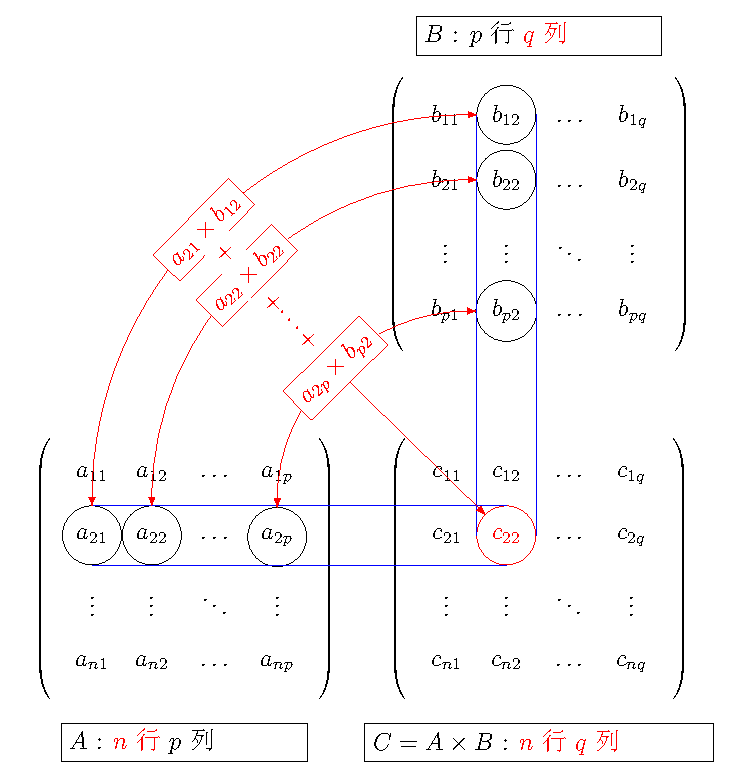
\includegraphics[scale=0.75]{figures/matrix-multiplication.pdf}
    \caption{}
\end{figure}

\begin{example}
    设 $\vb*{A}=\begin{pmatrix}
            a_{11} & a_{12} \\
            a_{21} & a_{22} \\
            a_{31} & a_{32} \\
        \end{pmatrix}$,
    $\vb*{B}=\begin{pmatrix}
            b_1 & 0   \\
            0   & b_2
        \end{pmatrix}$,
    $\vb*{C}=\begin{pmatrix}
            c_1 & 0   & 0   \\
            0   & c_2 & 0   \\
            0   & 0   & c_3
        \end{pmatrix}$, 求 $\vb*{AB}$ 和 $\vb*{CA}$.
\end{example}
\begin{solution}
    $\vb*{AB}=\begin{pmatrix}
            a_{11} & a_{12} \\
            a_{21} & a_{22} \\
            a_{31} & a_{32} \\
        \end{pmatrix}\begin{pmatrix}
            b_1 & 0   \\
            0   & b_2
        \end{pmatrix}=\begin{pmatrix}
            a_{11}b_1 & a_{12}b_2 \\
            a_{21}b_1 & a_{22}b_2 \\
            a_{31}b_1 & a_{32}b_2
        \end{pmatrix}$; 同理
    $\vb*{CA}=\begin{pmatrix}
            c_1a_{11} & c_1a_{12} \\
            c_2a_{21} & c_2a_{22} \\
            c_3a_{31} & c_3a_{32}
        \end{pmatrix}$
\end{solution}

\begin{example}
    设 $\vb*{A}$ 是 4 阶方阵, $\vb*{B}$ 是 5 阶方阵, 且 $|\vb*{A}|=2,|\vb*{B}|=-2$, 求 $|-|\vb*{A}|\vb*{B}|$ 与 $|-|\vb*{B}|\vb*{A}|$.
\end{example}
\begin{solution}
    $|-|\vb*{A}|\vb*{B}|=|-2\vb*{B}|=(-2)^{5}|\vb*{B}|=64$, $|-|\vb*{B}|\vb*{A}|=|2\vb*{A}|=2^4|\vb*{A}|=32.$
\end{solution}

\begin{example}
    设 $\vb*{A},~\vb*{B}$ 均为 3 阶矩阵, 满足 $\vb*{AB}+2\vb*{A}+\vb*{B}+\vb*{E}=\vb*{O}$,
    若 $|\vb*{B}|=\mqty|1&2&0\\1&2&0\\1&2&1|$, 求 $|\vb*{A}+\vb*{E}|.$
\end{example}
\begin{solution}
    对 $\vb*{AB}+2\vb*{A}+\vb*{B}+2\vb*{E}$ 使用多项式除法, 得 $$\vb*{AB}+2\vb*{A}+\vb*{B}+2\vb*{E}=(\vb*{A}+\vb*{E})(\vb*{B}+2\vb*{E})=\vb*{E}\Rightarrow|\vb*{A}+\vb*{E}|=\dfrac{1}{|\vb*{B}+2\vb*{E}|}=\dfrac{1}{30}.$$
\end{solution}

\subsection{方阵的幂}

\begin{definition}[方阵的幂]
    对 $ n $ 阶方阵 $ A $, 定义
    $\displaystyle\vb*{A}^{k}=\underbrace{\vb*{A} \cdot \vb*{A} \cdot \cdots \cdot \vb*{A}}_{k \text{个}}$,
    称为 $ \vb*{A} $ 的 $ k $ 次幂.
\end{definition}

\begin{example}
    设 $\vb*{A}=\mqty(\dfrac{2}{3}&-\dfrac{1}{3}&-\dfrac{1}{3}\\[6pt]-\dfrac{1}{3}&\dfrac{2}{3}&-\dfrac{1}{3}\\[6pt]-\dfrac{1}{3}&-\dfrac{1}{3}&\dfrac{2}{3})$, 求 $\vb*{A}^9$.
\end{example}
\begin{solution}
    $\vb*{A}^2=\mqty(\dfrac{2}{3}&-\dfrac{1}{3}&-\dfrac{1}{3}\\[6pt]-\dfrac{1}{3}&\dfrac{2}{3}&-\dfrac{1}{3}\\[6pt]-\dfrac{1}{3}&-\dfrac{1}{3}&\dfrac{2}{3})^{2}=\dfrac{1}{9}\mqty(6&-3&-3\\-3&6&-3\\-3&-3&6)=\vb*{A}$, 因此 $\vb*{A}^9=\vb*{A}\qty(\vb*{A}^2)^4=\vb*{A}\vb*{A}^4=\vb*{A}\qty(\vb*{A}^2)^2=\vb*{A}^2=\vb*{A}.$
\end{solution}

\subsubsection{利用幂零矩阵求解}

\begin{example}
    设 $\vb*{A}=\mqty(0&1&2&3\\0&0&2&3\\0&0&0&3\\0&0&0&0)$, 求解 $\vb*{A}^n.$
\end{example}
\begin{solution}
    因为 $\vb*{A}^4=\vb*{O}$, 并且
    \begin{flalign*}
        \vb*{A}^2=\mqty(0 & 1 & 2 & 3 \\0&0&2&3\\0&0&0&3\\0&0&0&0)\cdot\mqty(0&1&2&3\\0&0&2&3\\0&0&0&3\\0&0&0&0)=\mqty(0&0&2&9\\0&0&0&6\\0&0&0&0\\0&0&0&0)\\
        \vb*{A}^3=\mqty(0 & 0 & 2 & 9 \\0&0&0&6\\0&0&0&0\\0&0&0&0)\cdot \mqty(0&1&2&3\\0&0&2&3\\0&0&0&3\\0&0&0&0)=\mqty(0&0&2&9\\0&0&0&6\\0&0&0&0\\0&0&0&0)
    \end{flalign*}
\end{solution}

\subsubsection{利用方阵的迹求解}

\begin{theorem}[秩一矩阵的幂]
    当 $\vb*{A}$ 为方阵且秩 $\rank\vb*{A}=1$, 则 $\vb*{A}^n=\qty[\tr(\vb*{A})]^{n-1}\vb*{A}$.
\end{theorem}

\begin{example}
    设 $\vb*{A}=\mqty(a&b&c&d\\2a&2b&2c&2d\\3a&3b&3c&3d\\4a&4b&4c&4d)~  (a,b,c,d)$ 不全为 0, 求解 $\vb*{A}^n.$
\end{example}
\begin{solution}
    显然 $\rank\vb*{A}=1$, 则 $$\vb*{A}^n=\qty[\tr(\vb*{A})]^{n-1}\vb*{A}=(a+2b+3c+4d)^{n-1}\vb*{A}.$$
\end{solution}

\begin{example}
    设 $\vb*{A}=\mqty(0&0&1\\0&1&0\\1&0&0)$, 已知矩阵 $\vb*{B}$ 与矩阵 $\vb*{A}$ 相似, 求
    $\rank(\vb*{B}-2\vb*{E})+\rank(\vb*{B}-\vb*{E})$, 及 $(\vb*{A}-\vb*{E})^n$, $n$ 为大于 1 的正整数.
\end{example}
\begin{solution}
    因为 $\vb*{B}\sim\vb*{A}$, 所以
    \begin{flalign*}
        \rank(\vb*{B}-2\vb*{E})+\rank(\vb*{B}-\vb*{E}) & =\rank(\vb*{A}-2\vb*{E})+\rank(\vb*{A}-\vb*{E})=\rank\mqty(-2 & 0 & 1 \\0&-1&0\\1&0&-2)+\rank\mqty(-1&0&1\\0&0&0\\1&0&-1)\\
                                                       & =3+1=4
    \end{flalign*}
    因为 $\rank(\vb*{A}-\vb*{E})=1$, 所以 $(\vb*{A}-\vb*{E})^n=\qty[\tr(\vb*{A}-\vb*{E})\vb*{A}]^{n-1}(\vb*{A}-\vb*{E})=(-2)^{n-1}\mqty(-1&0&1\\0&0&0\\1&0&-1).$
\end{solution}

\subsubsection{利用二项式展开求解}

\begin{example}
    设 $\vb*{A}=\begin{pmatrix}
            1 & 3 \\
            0 & 1
        \end{pmatrix}$, 求 $\vb*{A}^n$.
\end{example}
\begin{solution}
    由 $\vb*{A}=\begin{pmatrix}
            1 & 3 \\
            0 & 1
        \end{pmatrix}=\begin{pmatrix}
            1 & 0 \\
            0 & 1
        \end{pmatrix}+\begin{pmatrix}
            0 & 3 \\
            0 & 0
        \end{pmatrix}=\vb*{E}+\vb*{B}$, 而
    $\displaystyle\vb*{B}^2=\begin{pmatrix}
            0 & 3 \\
            0 & 0
        \end{pmatrix}\begin{pmatrix}
            0 & 3 \\
            0 & 0
        \end{pmatrix}=\mathrm{0}$,
    所以当 $k\geqslant2$ 时, 有 $\vb*{B}^k=\mathrm{0}$,
    而单位矩阵 $\vb*{E}$ 与任意矩阵可换, 由二项式定理, 得
    \begin{flalign*}
        \vb*{A}^n & =(\vb*{E}+\vb*{B})^n=\sum_{k=0}^{n}\mathrm{C}_n^k\vb*{E}^{n-k}\vb*{B}^k=\vb*{E}^n+\mathrm{C}_n^1\vb*{E}^{n-1}B \\
                  & =\begin{pmatrix}
                         1 & 0 \\
                         0 & 1
                     \end{pmatrix}+n\begin{pmatrix}
                                        1 & 0 \\
                                        0 & 1
                                    \end{pmatrix}\begin{pmatrix}
                                                     0 & 3 \\
                                                     0 & 0
                                                 \end{pmatrix}=\begin{pmatrix}
                                                                   1 & 3n \\
                                                                   0 & 1
                                                               \end{pmatrix}.
    \end{flalign*}
\end{solution}

\begin{example}[2002 复旦大学]
    证明: $$\begin{pmatrix}
            \dfrac{3}{2} & -\dfrac{1}{2} \\[6pt]
            \dfrac{1}{2} & \dfrac{1}{2}
        \end{pmatrix}^{100}=\begin{pmatrix}
            51 & -50 \\
            50 & -49
        \end{pmatrix}.$$
\end{example}
\begin{proof}[{\songti \textbf{证}}]
    注意到 \begin{flalign*}
        \begin{pmatrix}
            \dfrac{3}{2} & -\dfrac{1}{2} \\[6pt]
            \dfrac{1}{2} & \dfrac{1}{2}
        \end{pmatrix}=\begin{pmatrix}
                          1 & 0 \\
                          0 & 1
                      \end{pmatrix}+\begin{pmatrix}
                                        \dfrac{1}{2} & -\dfrac{1}{2} \\[6pt]
                                        \dfrac{1}{2} & -\dfrac{1}{2}
                                    \end{pmatrix}=\begin{pmatrix}
                                                      1 & 0 \\
                                                      0 & 1
                                                  \end{pmatrix}+\begin{pmatrix}
                                                                    \dfrac{1}{2} \\[6pt]
                                                                    \dfrac{1}{2}
                                                                \end{pmatrix}(1,-1) =\vb*{E}+\vb*{\alpha}\vb*{\beta}^{\top}
    \end{flalign*}
    其中 $\vb*{E}$ 是二阶单位矩阵, $\vb*{\alpha}=\qty(\dfrac{1}{2},\dfrac{1}{2})^{\top}$, $\vb*{\beta}=(1,-1)^{\top}$, 并且 $\vb*{\beta}\vb*{\alpha}^T=0$, 所以
    $$\qty(\vb*{\alpha\beta}^\top)^2=\qty(\vb*{\alpha\beta}^{\top})\qty(\vb*{\alpha\beta}^{\top})=\vb*{\alpha}\qty(\vb*{\beta}^{\top}\vb*{\alpha})\vb*{\beta}^{\top}=\vb*{O}$$
    于是 \begin{flalign*}
        \begin{pmatrix}
            \dfrac{3}{2} & -\dfrac{1}{2} \\[6pt]
            \dfrac{1}{2} & \dfrac{1}{2}
        \end{pmatrix}^{100} & =\qty(\vb*{E}+\vb*{\alpha}\vb*{\beta}^{\top})^{100}=\sum_{k=0}^{100}\mathrm{C}_{100}^k\qty(\vb*{\alpha\beta}^\top)^k=\vb*{E}+100\vb*{\alpha\beta}^{\top} \\
                                             & =\begin{pmatrix}
                                                    1 & 0 \\
                                                    0 & 1
                                                \end{pmatrix}+100\begin{pmatrix}
                                                                     1 \\1
                                                                 \end{pmatrix}(1,-1)=\begin{pmatrix}
                                                                                         51 & -50 \\
                                                                                         50 & -49
                                                                                     \end{pmatrix}.
    \end{flalign*}
\end{proof}

\subsection{分块矩阵}

\begin{theorem}[分块矩阵的加减法]
    若矩阵 $ \vb*{A} $ 与矩阵 $ \vb*{B} $ 有相同的行数和列数, 且有
    $$\vb*{A}=\mqty(\vb*{A}_{11} & \cdots & \vb*{A}_{1 r} \\
        \vdots & & \vdots \\
        \vb*{A}_{s 1} & \cdots & \vb*{A}_{s r})
        , \quad \vb*{B}=\mqty(\vb*{B}_{11} & \cdots & \vb*{B}_{1 r} \\
        \vdots & & \vdots \\
        \vb*{B}_{s 1} & \cdots & \vb*{B}_{s r})$$
    其中 $ \vb*{A}_{i j} $ 与 $ \vb*{B}_{i j} $ 有相同的行数和列数, 则
    $$\vb*{A} \pm \vb*{B}=\mqty(\vb*{A}_{11} \pm \vb*{B}_{11}   & \cdots & \vb*{A}_{1 r} \pm \vb*{B}_{1 r} \\
        \vdots                                        &        & \vdots                                        \\
        \vb*{A}_{s 1} \pm \vb*{B}_{s 1} & \cdots & \vb*{A}_{s r} \pm \vb*{B}_{s r}).$$
\end{theorem}

\begin{theorem}[分块矩阵的数乘]
    设矩阵 $ \vb*{A}=\mqty(\vb*{A}_{11} & \cdots & \vb*{A}_{1 r} \\ \vdots & & \vdots \\ \vb*{A}_{s 1} & \cdots & \vb*{A}_{s r})$, $\lambda $ 为数, 则
    $$\lambda  \vb*{A}=\mqty(\lambda  \vb*{A}_{11} & \cdots & \lambda  \vb*{A}_{1 r} \\
        \vdots & & \vdots \\
        \lambda  \vb*{A}_{s 1} & \cdots & \lambda  \vb*{A}_{s r}).$$
\end{theorem}

\begin{theorem}[分块矩阵的乘法]
    若 $ \vb*{A} $ 为 $ m \times l $ 矩阵, $ \vb*{B} $ 为 $ l \times n $ 矩阵, 且
    $$\vb*{A}=\mqty(\vb*{A}_{11}  & \cdots & \vb*{A}_{1 t} \\
        \vdots        &        & \vdots        \\
        \vb*{A}_{s 1} & \cdots & \vb*{A}_{s t})
        , \quad \vb*{B}=\mqty(\vb*{B}_{11}  & \cdots & \vb*{B}_{1 r} \\
        \vdots        &        & \vdots        \\
        \vb*{B}_{t 1} & \cdots & \vb*{B}_{t r})$$
    其中 $ \vb*{A}_{i 1}, \vb*{A}_{i 2}, \cdots, \vb*{A}_{i i} $ 的列数分别与 $ \vb*{B}_{1 j}, \vb*{B}_{2 j}, \cdots, \vb*{B}_{i j} $ 的行数相等, 则
    $$\vb*{A B}=\mqty(C_{11}  & \cdots & C_{1 r} \\
        \vdots  &        & \vdots  \\
        C_{s 1} & \cdots & C_{s r})$$
    其中 $ \vb*{C}_{i j}=\displaystyle \sum_{k=1}^{t} \vb*{A}_{i k} \vb*{B}_{k j}(i=1, \cdots, s ; j=1, \cdots, r) $.
\end{theorem}

\begin{theorem}[分块矩阵的转置]
    设矩阵 $ \vb*{A}=\mqty(\vb*{A}_{11} & \cdots & \vb*{A}_{1 r} \\ \vdots & & \vdots \\ \vb*{A}_{s 1} & \cdots & \vb*{A}_{s r})
    $, 则 $ \vb*{A}^{\top}=\mqty(\vb*{A}_{11}^{\top} & \cdots & \vb*{A}_{s 1}^{\top} \\ \vdots & & \vdots \\ \vb*{A}_{1 r}^{\top} & \cdots & \vb*{A}_{s r}^{\top}) $.
\end{theorem}

\begin{theorem}[分块矩阵的行列式]
    设 $ \vb*{A}=\left(\begin{array}{llll}\vb*{A}_{1} & & & \\ & \vb*{A}_{2} & & \\ & & \ddots & \\ & & & A_{m}\end{array}\right) $, 其中 $ \vb*{A}_{i}(i=1,2, \cdots, m) $ 都是方阵, 则
          $$|\vb*{A}|=\left|\vb*{A}_{1}\right|\left|\vb*{A}_{2}\right| \cdots\left|\vb*{A}_{m}\right|, \quad \vb*{A}^{n}=\left(\begin{array}{llll}
                      \vb*{A}_{1}^{n} &                 &        &                 \\
                                      & \vb*{A}_{2}^{n} &        &                 \\
                                      &                 & \ddots &                 \\
                                      &                 &        & \vb*{A}_{m}^{n}
                  \end{array}\right) .$$
\end{theorem}

\subsection{Carlson 不等式及其应用}

\begin{theorem}[Carlson 不等式]
    对于 $n\times m$ 矩阵
    $$\begin{pmatrix}
            a_{11} & a_{12} & \dots  & a_{1m} \\
            a_{21} & a_{22} & \dots  & a_{2m} \\
            \vdots & \vdots & \ddots & \vdots \\
            a_{n1} & a_{n2} & \dots  & a_{nm} \\
        \end{pmatrix}$$
    其中 $a_{ij}\geqslant0~ (i=1,2,\cdots,n,j=1,2,\cdots,m)$, 则
    $$\qty[\prod_{j=1}^{m}\qty(\sum_{i=1}^{n}a_{ij})]^{\frac{1}{m}}\geqslant \sum_{i=1}^{n}\qty(\prod_{j=1}^{m}a_{ij})^{\frac{1}{m}}$$
    其中, 等号成立的充要条件是至少有一列数都是 0 或所有行中的数对应成比例.
\end{theorem}
\begin{proof}[{\songti \textbf{证}}]
    记 $\displaystyle A_j = \sum_{i=1}^{n}a_{ij}~ (j=1,2,\cdots,m),~G_j=\prod_{j=1}^{m}a_{ij}~ (i=1,2,\cdots,n)$, 
    若某个 $A_j=0$, 则由 $a_{ij}\geqslant 0~ (i=1,2,\cdots,n)$, 得 $$a_{1j}=a_{2j}=\cdots=a_{nj}=0$$
    此时, $G_1=G_2=\cdots=G_n=0$, 从而 $$\qty[\prod_{j=1}^{m}\qty(\sum_{i=1}^{n}a_{ij})]^{\frac{1}{m}}=\sum_{i=1}^{n}\qty(\prod_{j=1}^{m}a_{ij})^{\frac{1}{m}}$$
    若所有 $A_j>0$, 由均值不等式得 $$\dfrac{a_{i1}}{A_1}+\dfrac{a_{i2}}{A_2}+\cdots+\dfrac{a_{im}}{A_m}\geqslant m\qty(\dfrac{\displaystyle\prod_{j=1}^{m}a_{ij}}{\displaystyle\prod_{j=1}^{m}A_j})^{\frac{1}{m}}~ (i=1,2,\cdots,n)$$
    将以上 $n$ 个不等式相加得
    $$m\geqslant m\sum_{i=1}^{n}\qty(\dfrac{\displaystyle\prod_{j=1}^{m}a_{ij}}{\displaystyle\prod_{j=1}^{m}A_j})^{\frac{1}{m}}=m\dfrac{\displaystyle\sum_{i=1}^{n}G_i^{\frac{1}{m}}}{\qty(\displaystyle\prod_{j=1}^{m}A_j)^{\frac{1}{m}}}$$
    等号成立的充要条件是至少有一列数都是 0 或 $\dfrac{a_{i1}}{A_1}=\dfrac{a_{i2}}{A_2}=\cdots=\dfrac{a_{im}}{A_m}$.
\end{proof}

\begin{example}
    已知 $a,b,c>0$, 证明: $$\qty(a^2+ab+b^2)\qty(b^2+bc+c^2)\qty(c^2+ca+a^2)\geqslant (ab+bc+ca)^3.$$
\end{example}
\begin{proof}[{\songti \textbf{证}}]
    构造 $3\times 3$ 矩阵
    $$\begin{pmatrix}
            a^2 & c^2 & ca  \\
            ab  & b^2 & a^2 \\
            b^2 & bc  & c^2
        \end{pmatrix}$$
    由 Carlson 不等式得证.
\end{proof}

\begin{example}
    已知 $a,b,c>0$, $a^2+b^2+c^2=14$, 求证: $a^5+\dfrac{b^5}{8}+\dfrac{c^5}{27}\geqslant 14.$
\end{example}
\begin{proof}[{\songti \textbf{证}}]
    构造 $3\times 5$ 矩阵
    $$\begin{pmatrix}
            a^5             & a^5             & 1 & 1 & 1 \\[6pt]
            \dfrac{b^5}{8}  & \dfrac{b^5}{8}  & 4 & 4 & 4 \\[6pt]
            \dfrac{c^5}{27} & \dfrac{c^5}{27} & 9 & 9 & 9
        \end{pmatrix}$$
    由 Carlson 不等式得, 
    \begin{flalign*}
        \qty[\qty(a^5+\dfrac{b^5}{8}+\dfrac{c^5}{27})^2(1+4+9)^3]^{\frac{1}{5}} & \geqslant \qty(a^5\cdot a^5\cdot 1^3)^{\frac{1}{5}}+\qty(\dfrac{b^5}{8}\cdot \dfrac{b^5}{8}\cdot 4^3)^{\frac{1}{5}}+\qty(\dfrac{c^5}{27}\cdot\dfrac{c^5}{27}\cdot 9^3)^{\frac{1}{5}} \\
        \qty[\qty(a^5+\dfrac{b^5}{8}+\dfrac{c^5}{27})^214^3]^{\frac{1}{5}}      & \geqslant a^2+b^2+c^2=14
    \end{flalign*}
    整理得证 $a^5+\dfrac{b^5}{8}+\dfrac{c^5}{27}\geqslant 14.$
\end{proof}

\begin{example}
    已知 $a_i>0~ (i=1,2,\cdots,n),~n\geqslant 2$, 且 $\displaystyle\sum_{i=1}^{n}a_i=1$, 
    证明: $\displaystyle\sum_{i=1}^{n}\dfrac{a_i}{2-a_i}\geqslant \dfrac{n}{2n-1}.$
\end{example}
\begin{proof}[{\songti \textbf{证}}]
    原不等式等价为 $$\sum_{i=1}^{n}\dfrac{2}{2-a_i}\geqslant \dfrac{2n^2}{2n-1}$$
    为此, 构造 $n\times 2$ 矩阵
    $$\begin{pmatrix}
            \dfrac{2}{2-a_1} & 2-a_1  \\[6pt]
            \dfrac{2}{2-a_2} & 2-a_2  \\[6pt]
            \vdots           & \vdots \\[6pt]
            \dfrac{2}{2-a_n} & 2-a_n
        \end{pmatrix}$$
    由 Carlson 不等式得, 
    \begin{flalign*}
        \qty[\qty(\sum_{i=1}^{n}\dfrac{2}{2-a_i})\sum_{i=1}^{n}(2-a_i)]^{\frac{1}{2}}\geqslant \sqrt{2}n\Rightarrow\qty(\sum_{i=1}^{n}\dfrac{2}{2-a_i})(2n-1)\geqslant 2n^2
    \end{flalign*}
    整理得证 $\displaystyle\sum_{i=1}^{n}\dfrac{a_i}{2-a_i}\geqslant \dfrac{n}{2n-1}.$
\end{proof}

\begin{example}
    (第 36 届 IMO) 设 $a,b,c>0$, 且 $abc=1$, 证明: $\dfrac{1}{a^3(b+c)}+\dfrac{1}{b^3(c+a)}+\dfrac{1}{c^3(a+b)}\geqslant\dfrac{3}{2}.$
\end{example}
\begin{proof}[{\songti \textbf{证}}]
    原不等式等价为 $$\dfrac{b^2c^2}{a(b+c)}+\dfrac{a^2c^2}{b(c+a)}+\dfrac{a^2b^2}{c(a+b)}$$
    构造 $3\times 2$ 矩阵
    $$\begin{pmatrix}
            \dfrac{b^2c^2}{a(b+c)} & a(b+c) \\[6pt]
            \dfrac{a^2c^2}{b(a+c)} & b(a+c) \\[6pt]
            \dfrac{a^2b^2}{c(a+b)} & c(a+b)
        \end{pmatrix}$$
    由 Carlson 不等式得, 
    \begin{flalign*}
        \qty{\qty[\dfrac{b^2c^2}{a(b+c)}+\dfrac{a^2c^2}{b(c+a)}+\dfrac{a^2b^2}{c(a+b)}]\cdot2(ab+bc+ca)}^{\frac{1}{2}} & \geqslant ab+bc+ca                                                                      \\
        \dfrac{b^2c^2}{a(b+c)}+\dfrac{a^2c^2}{b(c+a)}+\dfrac{a^2b^2}{c(a+b)}                                           & \geqslant \dfrac{1}{2}(ab+bc+ca)\geqslant \dfrac{3}{2}\sqrt[3]{a^2b^2c^2}=\dfrac{3}{2}.
    \end{flalign*}
\end{proof}